\chapter{WSTĘP}
\section{Wstęp}

Celem projektu było stworzenie systemu do analizy struktury sieci WWW uczelni zagranicznej. Główne zadanie polegało na zaprojektowaniu i zaimplementowaniu robota internetowego, który przegląda zasoby w obrębie wskazanej domeny, zapisuje je lokalnie, a następnie buduje skierowany graf połączeń pomiędzy stronami. Uzyskany graf stanowił podstawę do przeprowadzenia dalszych analiz topologicznych. Wybrana uczelnia zagraniczna to Uniwersytet Maltański \url{https://www.um.edu.mt/}.

Crawler został zaimplementowany w języku Python z wykorzystaniem takich bibliotek jak \texttt{threading}, \texttt{queue}, \texttt{networkx}, \texttt{tqdm} oraz standardowych narzędzi do parsowania stron. Obsługuje on wielowątkowe pobieranie dokumentów, przestrzega zasad \texttt{robots.txt} oraz automatycznie analizuje strukturę połączeń między stronami w czasie rzeczywistym.

\section{Opis działania crawlera}

Zaimplementowany crawler działa w oparciu o architekturę kolejki zadań i dynamicznie zarządzanych wątków. Działa w sposób asynchroniczny i dostosowuje liczbę aktywnych wątków w zależności od aktualnego obciążenia. Poniżej przedstawiono szczegóły działania:

\begin{itemize}
    \item \textbf{Inicjalizacja:} Crawler przyjmuje adres początkowy (URL) oraz maksymalną liczbę stron do odwiedzenia. Tworzona jest kolejka adresów oraz struktury do przechowywania odwiedzonych stron i grafu połączeń.
    
    \item \textbf{Zarządzanie wątkami:} Funkcja \texttt{run\_crawler()} odpowiada za dynamiczne uruchamianie nowych wątków w miarę potrzeb. Wątki są tworzone tylko wtedy, gdy kolejka zadań nie jest pusta i liczba aktywnych wątków nie przekracza zadeklarowanego limitu.
    
    \item \textbf{Wątek roboczy:} Każdy wątek wykonuje funkcję \texttt{child\_thread()}, która:
    \begin{itemize}
        \item sprawdza, czy dana strona może być pobrana (zgodność z \texttt{robots.txt}),
        \item pobiera stronę przy użyciu funkcji \texttt{download\_page()},
        \item parsuje zawartość HTML i wyciąga linki (\texttt{extract\_links()}),
        \item aktualizuje zbiór odwiedzonych stron i graf (z wykorzystaniem blokad synchronizujących \texttt{threading.Lock}).
    \end{itemize}

    \item \textbf{Kończenie pracy:} Crawler kończy działanie, gdy:
    \begin{itemize}
        \item osiągnięto maksymalną liczbę odwiedzonych stron,
        \item kolejka zadań jest pusta i nie ma aktywnych wątków.
    \end{itemize}
    Synchronizacja wątków odbywa się z wykorzystaniem mechanizmu \texttt{Condition}, co pozwala na usypianie i wybudzanie procesu głównego w zależności od sytuacji.

    \item \textbf{Wizualizacja postępu:} Podczas działania wyświetlany jest pasek postępu przy użyciu biblioteki \texttt{tqdm}, który pozwala śledzić liczbę przetworzonych stron.
\end{itemize}

\section{Wielowątkowość}

Crawler został uruchomiony z różną liczbą wątków: 1, 2, 4, 8 i 16, gdzie liczba odwiedzonych stron została ustawiona na przynajmniej 1000. Testy na wątkach przeprowadzono na mniejszej liczbie wierzchołków ze względu na czas działania programu, dla 3000 stron przedstawiałyby się one podobnie. Dla każdej konfiguracji zmierzono czas działania, a także zarejestrowano liczbę odwiedzonych wierzchołków i zbudowanych krawędzi w grafie.

\begin{table}[H]
\centering
\caption{Wyniki działania crawlera dla różnych liczby wątków dla przynajmniej 1000 stron}
\begin{tabular}{|c|c|c|c|}
\hline
\textbf{Liczba wątków} & \textbf{Czas (s)} & \textbf{Wierzchołki} & \textbf{Krawędzie} \\
\hline
1   & 2912.54 & 1000 & 55208 \\
2   & 1373.82 & 1000 & 54778 \\
4   & 731.47  & 1000 & 54684 \\
8   & 516.76  & 1001 & 53075 \\
16  & 387.61  & 1000 & 54182 \\
\hline
\end{tabular}
\end{table}

\begin{figure}[H]
    \centering
    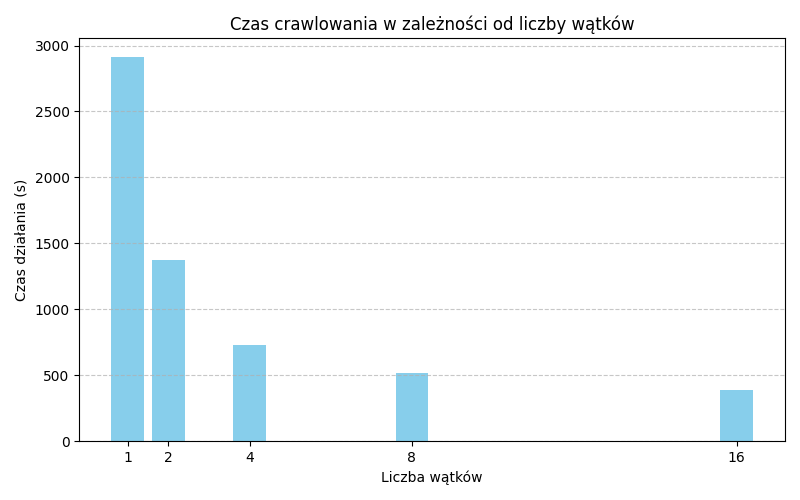
\includegraphics[width=\textwidth]{assets/img_61.png}
    \caption{Wykres czasu crawlowania w stosunku do liczby wątków dla przynajmniej 1000 stron.}
    \label{fig:watki}
\end{figure}

\subsection{Analiza wyników}

\begin{itemize}
    \item Zauważalny jest wyraźny spadek czasu działania wraz ze wzrostem liczby wątków. Przejście z 1 do 2 wątków skróciło czas ponad dwukrotnie.
    
    \item Kolejne wzrosty liczby wątków również przynoszą korzyści, jednak zgodnie z prawem malejących przychodów, różnice te stają się coraz mniejsze (np. różnica między 8 a 16 wątkami to tylko 129 s).
    
    \item Dla testu z 16 wątkami osiągnięto średnią prędkość pobierania około 0{,}39 sekundy na stronę.
\end{itemize}

\subsection{Wnioski}

Crawler bardzo dobrze skalował się w zakresie 1-8 wątków. Dalsze zwiększanie liczby wątków nadal poprawiało czas, lecz z mniejszym zyskiem. Możliwe wąskie gardła to:
\begin{itemize}
    \item ograniczenia sieciowe lub po stronie serwera,
    \item opóźnienia wynikające z synchronizacji wątków (blokady),
    \item zróżnicowana głębokość eksplorowanych ścieżek.
\end{itemize}

Optymalną liczbą wątków w tym środowisku wydaje się być 8 lub 16. Dlatego docelowo crawler został puszczony na 16 wątkach.


